%
% This template has been created by:
%   Pascal Bercher, 
%   - pascal.bercher@anu.edu.au, 
%   - https://bercher.net
%
% The newest version can be found on:
% https://gitlab.anu.edu.au/u1092535/latex-templates/
%
% Version number: 
%   Probably 1.08, but there's a chance it's actually
%   slightly newer and I just forgot to update this line. :)
%
% Version history:
%   Detailed change logs are provided in the file readme.txt.
%
% I was too lazy to put it under a specific license (will do
% so eventually; but might take me a few more years...), but
% you are still free to use and alter it. However, since I 
% put a *lot* of effort (and experience) in it, I insist on
% keeping my credentials in here (at the top), which give
% credit to me as an author. I explicitly forbid re-publishing
% my code (or content) until I put it under a specific license
% which would then clarify the rights. However, as said, *using*
% it is *of course* allowed, this is after all why I created it!
%
% Good luck with your thesis, and enjoy the journey  --  Pascal

\documentclass[a4paper,twoside,cleardoublepage=plain,bibliography=totoc]{scrbook}

\usepackage[a4paper]{geometry}                    % used for defining the title page

\usepackage{xurl}                                 % allows long URLs to break at any position
\usepackage[backref=page]{hyperref}               % defines style of references / links
\hypersetup{
linktocpage,                                      % in the table of contents, the numbers serve as links, not the entries
colorlinks  = true,                               % the items are colored instead of colored boxes around them
urlcolor    = cyan,
linkcolor   = red,
citecolor   = blue
}
% the following makes back references more appealing.
% Taken from: https://tex.stackexchange.com/questions/183702/formatting-back-references-in-bibliography-bibtex
\renewcommand*{\backref}[1]{}
\renewcommand*{\backrefalt}[4]{[%
\ifcase #1 Not cited.%
  \or Cited on page~#2.%
  \else Cited on pages #2.%
\fi]}




\usepackage{datetime}                                % to be able to print month & year on title page
  \newdateformat{monthonly}{\monthname[\THEMONTH]}
\usepackage{amssymb,amsthm,amsmath}                  % standard math packages; often used
\usepackage{graphicx}                                % allows including graphics
\usepackage{natbib}                                  % a specific citation style
\usepackage{floatrow}                                % allows to place a caption next to a figure
  \floatsetup[table]{capposition=top}                 % forces table captions to appear on top.
\usepackage[linesnumbered,ruled,vlined]{algorithm2e} % used for depicting algorithms
\usepackage{booktabs}                                % for tables that actually look nice!
\usepackage{paralist}                                % provides compactitem, a more compact itemize
\usepackage{titlesec}                                % used to add those horizontal lines around chapter package; see defs below.
\usepackage[standardsections]{scrhack}                % fixes an error causes by loading titlesec for class scrbook
\usepackage{parskip}                                 % when this is included, no indentations are used for new paragraphs,
                                                     % and instead paragraphs are separated by a small distance between them


% [requires titlesec]
% Surrounds all chapter titles by lines,
\titleformat{\chapter}[display]
{\bfseries\huge}
{\filleft\Large\chaptertitlename~\thechapter}
{3ex}
{\titlerule\vspace{1.5ex}\filright}
[\vspace{1ex}\titlerule]

% fixes a compilation errror that otherwise occurs in combination with scrbook
% see https://tex.stackexchange.com/questions/625083/adding-horizontal-line-before-and-after-chapter-heading-in-scrbook
% \titleformat{\section}
%  {\normalfont\Large\bfseries}{\thesection}{1em}{}
% \titleformat{\subsection}
%  {\normalfont\large\bfseries}{\thesubsection}{1em}{}
% \titleformat{\subsubsection}
%  {\normalfont\normalsize\bfseries}{\thesubsubsection}{1em}{}
 

 

% Set your individual data for the title page in the configuration file
% AND DON'T SCREW UP THIS DATA! You should know, for example, whether it's
% an Honours thesis or not, or in which semester it is running.

% Set your name:
%  (Well, your name.)
\newcommand{\AuthorName} {Xin Lu}


% Set the title of your work:
%  (Choose an informative and interesting title.)
\newcommand{\ProjectTitle} {Template for Project Reports}


% Set which titlepage layout you prefer. Both provide the exact same
% information, they only differ in design to give you a bit of individuality
%  (change second line accordingly)
\newif\ifStandardTitle % do not delete this part!
\StandardTitletrue     % comment out (or use \StandardTitlefalse)
                       % to switch to an alternative title page layout


% Set the name of your school:
%  (School of Computing, School of Engineering,
%   or School of Cybernetics)
\newcommand{\School} {School of Computing}


% Set the name of your college:
%  (However your College is called.)
\newcommand{\College} {College of Engineering, Computing and Cybernetics (CECC)}


% Set your project points:
%  (6 or 12)
%  can be ignored for Honours theses, since those are always 24 pt anyway
%  and hence set automatically
\newcommand{\ProjectPoints} {6}


% Set whether it's an Honours thesis:
%  (change second line accordingly)
\newif\ifHonoursThesis % do not delete this part!
\HonoursThesistrue     % or \HonoursThesisfalse or comment out


% Set your semester:
%  (S1 or S2 or S1/S2 or S2/S1 or Summer)
\newcommand{\Semester} {S2/S1}


% Set your year:
%  (YYYY or YYYY--YYYY in case of S2/S1)
\newcommand{\Year} {2023--2024}


% Set your degree:
%  (Whatever your degree is called.)
%  (Only required if Honours = true)
\newcommand{\Degree} {Bachelor of Advanced Computing}


% Set your course code and name:
%  (Whatever your course code and name is.)
%  (Only required if Honours = false)
\newcommand{\CourseCode} {COMP1234}
\newcommand{\CourseName} {Course Name}


% Set name of first supervisor:
%   (Whatever her or his name is.)
\newcommand{\FirstSupervisor} {Dr.\ FirstName LastName}


% Set whether there's a second supervisor:
%  (change second line accordingly)
\newif\ifTwoOrMoreSupervisors % do not delete this part!
\TwoOrMoreSupervisorstrue     % or \TwoOrMoreSupervisorsfalse or comment out


% Set name of second supervisor:
%  (Whatever her or his name is.)
%  (Only required if TwoSupervisors = true)
\newcommand{\SecondSupervisor} {%
Dr.\ Second Supervisor
%\\Prof.\ Dr.\ Third Supervisor (if there is any)
%\\Prof.\ Dr.\ Dr.\ Fourth Supervisor (if we need four, five, etc.)
}
                             % to specify data used in the title page

% define your own macros here
\definecolor{vlightgray}{gray}{0.95}
\newcommand{\comptitle}[2]{\multicolumn{1}{c#1}{\cellcolor{vlightgray}#2}}

\newcommand{\Eff} {\ensuremath{\mathit{eff}}}  % example command without arguments
\newcommand{\Pre} {\ensuremath{\mathit{pre}}}  % (again)

% Note that you can easily specify arguments:
% \newcommand{\someMacro}[2] {Argument 1: #1, Argument 2: #2} % example command with two arguments
% you use it via \someMacro{Hello}{World!}


% the following commands are being provided by the amsthm package
% the first parameter states the new environmet's name that can be
% used (due to this definition here) and the second the name that
% will appear in the PDF document
\theoremstyle{definition}
\newtheorem{definition}{Definition}   % well, a formal definition!
\theoremstyle{plain}
\newtheorem{prop}{Proposition} % like a theorem, but less important or evolved
\newtheorem{lem}{Lemma}        % used within a proof of a theorem
\newtheorem{thm}{Theorem}      % well, a theorem! :) important and evolved
\newtheorem{cor}{Corollary}    % basically either a proposition or theorem,
                               %  but one that follows from another theorem.
% There's a lot you can configure about the appearance. If interested,
% open the manual of amsthm or google for tutorials etc. on that package

% the following add a symbol to the definition environment to make it more
% clear when a definition ends (as there is no difference in fonts!). From:
% https://tex.stackexchange.com/questions/226334/change-a-amsthm-theorem-ending
\newcommand{\xqed}[1]{%
    \leavevmode\unskip\penalty9999 \hbox{}\nobreak\hfill
    \quad\hbox{\ensuremath{#1}}}
\newcommand{\Endofdef}{\xqed{\blacksquare}}
\newenvironment{defn}[1]{%
    \begin{definition}#1}{%
    \Endofdef\end{definition}%
}
\newcommand{\provtrans}[4]{#1 \;\xrightarrow[{#3}]{#2}\;#4}

%\definecolor{sgreen}{rgb}{0,0.3,0}
\newcommand{\api}{applied pi-calculus}
\newcommand{\ccpic}{concurrent constraint pi-calculus}
\newcommand{\ccpi}{CC-Pi calculus}
\newcommand{\efc}{explicit fusion calculus}
\newcommand{\pif}{pi-F}
%\newcommand{\spic}{spi calculus}
%\newcommand{\Api}{Applied pi-Calculus}
%\newcommand{\picalculus}{pi calculus}
%\newcommand{\Picalculus}{Pi calculus}
\newcommand{\psicalculus}{psi-calculus}
\newcommand{\psicalculi}{psi-calculi}
\newcommand{\Psicalculi}{Psi-calculi}
\newcommand{\ve}[1]{\widetilde{#1}}
\newcommand{\0}{\emptyset}
\newcommand{\Set}[2][]{\{ #1 #2 #1 \}}
\newcommand{\POWERSET}{\mathcal{P}}
\newcommand{\powerset}[1]{\POWERSET(#1)}
\newcommand{\POWERFIN}{\POWERSET_{\!\text{fin}}}
\newcommand{\powerfin}[1]{\POWERFIN(#1)}
% \newcommand{\defn}{\;\mathrm{\triangleq}\;}
\newcommand{\apitransarrow}[1]{\goesto{#1}}
\newcommand{\apinottransarrow}[1]{\notgoesto{#1}}
\newcommand{\nottrans}[2]{#1 \; \apinottransarrow{#2}}
\newcommand{\compacttrans}[3]{#1 \apitransarrow{#2} #3}
\newcommand{\trans}[3]{#1 \; \apitransarrow{#2} \; #3}
\newcommand{\otrans}[3]{#1 \; \apitransarrow{#2}_o \; #3}
\newcommand{\attrans}[5]{#1 \; \apitransarrow{#2}_{#5}^{#4} \; #3}
\newcommand{\utrans}[3]{#1 \; \apitransarrow{#2}_U \; #3}
\newcommand{\transpi}[3]{#1 \; \apitransarrow{#2}_\pi \; #3}
\newcommand{\transapi}[3]{#1 \; \apitransarrow{#2}_{A\pi} \; #3}
\newcommand{\transs}[4]{#1~\xrightarrow[#3]{#2}~#4}
\newcommand{\sgto}[2]{\xrightarrow[#2]{#1}}
%\newcommand{\transnn}[4]{#1 \; \goesto{#2\;[#3]} \; #4}
%\newcommand{\transs}[3]{#1 \; \goesto{#2}_s \; #3}
%\newcommand{\transb}[3]{#1 \; \Sgoesto{#2} \; #3}
%\newcommand{\transc}[4]{#1 \; \xrightarrow[#3]{#2} \; #4}
%\newcommand{\transw}[3]{#1 \; \stackrel{#2}{\Longrightarrow} \; #3}
%\newcommand{\transws}[3]{#1 \; \stackrel{#2}{\Longrightarrow}_s \; #3}
%\newcommand{\outunit}[1]{\overline{#1}}

% Send
\newcommand{\sendtok}{\mbox{\rm \textbf{send}}}
\newcommand{\totok}{\mbox{\rm \textbf{to}}}
\newcommand{\outprefix}[2]{\sendtok\,#2\,\totok\,#1}
\newcommand{\outprefixpl}[3]{\outprefix{#1}{#2\sb{#3}}}
% Receive
\newcommand{\recvtok}{\mbox{\rm \textbf{receive}}}
\newcommand{\fromtok}{\mbox{\rm \textbf{from}}}
\newcommand{\intok}{\mbox{\rm \textbf{in}}}
\newcommand{\inprefixpi}[2]{\recvtok\,#2\,\fromtok\,#1}
\newcommand{\inprefixpl}[3]{\recvtok\,#2\,\intok\,\langle #3 \rangle\,\fromtok\,#1}

% Internal choice
\newcommand{\choosetok}{\mbox{\rm \textbf{choose}}}
\newcommand{\fortok}{\mbox{\rm \textbf{for}}}
\newcommand{\intchoiceprefix}[2]{\choosetok\,#2\,\fortok\,#1}
% External choice
\newcommand{\choosestok}{\mbox{\rm \textbf{chooses}}}
\newcommand{\ortok}{\mbox{\rm \textbf{or}}}

\newcommand{\extchoice}[3]{#1\,\choosestok\,\HOLConst{T}:\,#2\,\ortok\,\HOLConst{F}:#3}


\newcommand{\outprefixempty}[1]{\overline{#1}}
\newcommand{\outprefixpiF}[1]{\overline{#1}}
\newcommand{\outprefixcc}[2]{\outprefix{#1}{#2}}
\newcommand{\brinlabelempty}[1]{\underline{\text{\textrm{?}}#1}}
\newcommand{\brinlabel}[2]{\brinlabelempty{#1}\: #2}
\newcommand{\brbinlabel}[2]{\brinlabelempty{#1}(#2)}
\newcommand{\broutlabelempty}[2][p]{\overline{{\textrm{!}#2}}}
\newcommand{\broutlabel}[3][p]{\broutlabelempty[#1]{#2}\: #3}
\newcommand{\brbout}[4][p]{\broutlabelempty[#1]{#3}\:(\mathbf{\nu}#2) #4}
%\newcommand{\brbout}[3]{\broutlabelempty{#2}\:(\mathbf{\nu}#1) #3}
\newcommand{\binlabel}[2]{\underline{#1}(#2)}
\newcommand{\inlabel}[2]{\underline{#1}\: #2}
\newcommand{\inlabelpi}[2]{\leftarrow#1: #2}
\newcommand{\inlabelempty}[1]{\underline{#1}}
\newcommand{\inlabelpiF}[1]{\underline{#1}}
\newcommand{\inlabelcc}[2]{\inprefixcc{#1}{#2}}
\newcommand{\inlabelccb}[2]{\inprefixcc{#1}{(\nu #2)#2}}
\newcommand{\inlabellate}[3]{\underline{#1}(#3)}
\newcommand{\inlabelpm}[3]{\underline{#1}(\lambda #2) #3}
\newcommand{\outlabel}[2]{\rightarrow{}#1:#2}
\newcommand{\coutlabel}[3]{#1 \rightarrow #2: #3}
\newcommand{\intchlabel}[3]{\coutlabel{#1}{#2}{#3}}
\newcommand{\cinlabel}[3]{#2 \leftarrow #1: #3}
\newcommand{\outlabelpiF}[1]{\overline{#1}}
\newcommand{\outlabelempty}[1]{\overline{#1}}
\newcommand{\outlabelcc}[2]{\outprefixcc{#1}{#2}}
\newcommand{\outlabelccb}[2]{\outprefixcc{#1}{(\nu #2)#2}}
%\newcommand{\innn}[3]{\underline{#1} (#3)}
\newcommand{\inprefixshort}[2]{\underline{#1}(#2)}
\newcommand{\inprefixempty}[1]{\underline{#1}}
\newcommand{\inprefixpiF}[1]{\underline{#1}}
\newcommand{\inprefixcc}[2]{\underline{#1} #2}
\newcommand{\inprefixsym}[2]{#1(#2)}
\newcommand{\cendpoint}[4]{(#1, #2, #3) \rhd #4}
\newcommand{\pendpoint}[5]{(#1, #2, #3, #4) \rhd #5}
\newcommand{\brinprefix}[3]{\underline{\text{\textrm{?}}#1}(\lambda #2) #3}
\newcommand{\grossarrow}{\mathrel{\mathtt{-\!\!\!\!>}}}
\newcommand{\commprefix}[4]{#1 . #2  \grossarrow #3 . #4}
\newcommand{\commprefixsimp}[2]{#1 \grossarrow #2}
\newcommand{\selprefix}[3]{#1 \grossarrow #3[#2]}
\newcommand{\tell}[1]{\mathbf{tell}\; #1}
\newcommand{\ask}[1]{\mathbf{ask}\; #1}
%\newcommand{\lin}[3]{\underline{#1}(\lambda #2) #3}
\newcommand{\bout}[3]{\overline{#2}\:(\mathbf{\nu}#1) #3}
%\newcommand{\sbout}[3]{\overline{#1}(\mathbf{\nu}#2)#3}
\newcommand{\fuselabel}[2]{?#1\mbox{\scriptsize{=}}#2}
\newcommand{\fusion}[2]{#1\mbox{\scriptsize{=}}#2}
\newcommand{\datum}[1]{\langle #1\rangle}
%\newcommand{\oout}[2]{\mathbf{\exists}#2\overline{#1}\langle #2 \rangle}
%\newcommand{\inp}[2]{#1\langle #2 \rangle}
%\newcommand{\sinp}[3]{#1\:\lambda #2 #3}
%\newcommand{\sout}[2]{\overline{#1}#2}
%\newcommand{\binp}[2]{#1(#2)}
%\newcommand{\sbn}[1]{{\rm sbn}(#1)}
%\newcommand{\conds}{\triangleleft}
%\newcommand{\vareq}{\equiv_{\rm V}}
%\newcommand{\equivc}{\equiv_{c}}
%\newcommand{\equivn}{\equiv_{n}}
%\newcommand{\equivr}{\equiv_{r}}
%\newcommand{\equivs}{\equiv_{s}}
%\newcommand{\lequal}[1]{=_{#1}}
%\newcommand{\equations}{\mbox{\rm \bf \sf \small E}}
%\newcommand{\aframe}[1]{\mathcal{F}(#1)}
%\newcommand{\sframe}[1]{\mathcal{F}(#1)}
%\newcommand{\tframe}[1]{\mathcal{F}(#1)}
%\newcommand{\cframe}[1]{\mathcal{F}_\Phi(#1)}
%\newcommand{\fc}[1]{\mathcal{C}_F[#1]}
\newcommand{\frameof}[1]{\mathcal{F}(#1)}
%\newcommand{\ag}[1]{\mathcal{A}(#1)}
%\newcommand{\fradd}{\cup}
\newcommand{\frames}{\,\rhd\,}
%\newcommand{\sol}[1]{sol(#1)}
%\newcommand{\al}[2]{(\nu #2=#1)}
%\newcommand{\alias}[3]{\textbf{alias } \{{}^{#1}\!/\!{}_{#2}\} \textbf{ in }#3}
%\newcommand{\letin}[3]{\textbf{let } #2 = #1 \textbf{ in } #3}
%\newcommand{\sat}[2]{Sat_{#1}(#2)}
\newcommand{\res}[1]{(\mathbf{\nu}#1)}
%\newcommand{\resvar}[2]{(\mathbf{\nu}#1:#2)}
%\newcommand{\scope}[1]{\mathbf{\nu}#1}
%\newcommand{\fresh}[1]{\res{#1}}
\newcommand{\freshin}{\#}
%\newcommand{\notfreshin}{}
%\newcommand{\ground}[1]{ground(#1)}
%\newcommand{\constrains}{\triangleright}
%\newcommand{\lconstrains}{\triangleleft}
%\newcommand{\mappings}{\triangleright}
%\newcommand{\hooks}{\triangleleft}
%\newcommand{\och}{\wedge}
%\newcommand{\logicify}[1]{logicify(#1)}
\newcommand{\iftok}{\mbox{\textrm{\textbf{if}}}}
\newcommand{\thentok}{\mbox{\textrm{\textbf{then}}}}
\newcommand{\elsetok}{\mbox{\textrm{\textbf{else}}}}
\newcommand{\ifthel}[3]{\mbox{\iftok{} \ensuremath{#1} \thentok{} \ensuremath{#2} \elsetok{} \ensuremath{#3}}}
\newcommand{\fixc}[2]{\ensuremath{\mu #1. #2}}
\newcommand{\fixcall}[1]{#1}
\newcommand{\ifthen}[2]{\mbox{\iftok{} \ensuremath{#1} \thentok{} \ensuremath{#2}}}
% \newcommand{\letin}[1]{\mbox{\rm\ensuremath{\textbf{let } #1 \textbf{ in }}}}
\newcommand{\letin}[1]{\mbox{\textrm{\textbf{let }}\ensuremath{#1}\textrm{\textbf{ in }}}}
\newcommand{\letrecin}[2]{\mbox{\rm\ensuremath{\textbf{letrec } #1 \textbf{ in }
#2}}}
\newcommand{\closure}[2]{\mbox{\rm\ensuremath{\textbf{Cl } #1 \textbf{ in }
#2}}}
\newcommand{\letreconly}{\mbox{\rm\ensuremath{\textbf{letrec }}}}
\newcommand{\letonly}{\mbox{\rm\ensuremath{\textbf{let }}}}
\newcommand{\ci}[2]{#1:#2} % Case item
\newcommand{\cit}[1]{#1:} % Case item
%\newcommand{\caseelse}[2]{\textbf{case } #1 \textbf{ else } #2}
%\newcommand{\caseoelse}[2]{\textbf{case } #1 \text{ }[\textbf{else } #2]}
\ifdefined\case
\renewcommand{\case}[1]{\mbox{\rm\ensuremath{\textbf{case } #1}}}
\else
\newcommand{\case}[1]{\mbox{\rm\ensuremath{\textbf{case } #1}}}
\fi
\newcommand{\casesep}{\mathrel{[\hspace{-0.1ex}]}} %black box please?
\newcommand{\casen}{\mbox{\rm\ensuremath{\textbf{case\ }}}}
\newcommand{\boldword}[1]{\mbox{\rm\ensuremath{\textbf{#1}}}}
\newcommand{\caseonly}{\boldword{case}}
%\newcommand{\casesprod}[1]{\textbf{case}\casesep #1}
\newcommand{\pll}{\;|\;}
%\newcommand{\cpll}{\:\parallel\:}
%\newcommand{\vect}[1]{\langle #1 \rangle}
%\newcommand{\typeass}[3]{#1:\vect{#2;#3}}
%\newcommand{\tass}[2]{#1:#2}
%\newcommand{\typeassv}[3]{\tilde{#1}:\vect{\tilde{#2};\tilde{#3}}}
%\newcommand{\tassv}[2]{\tilde{#1}:\tilde{#2}}
%\newcommand{\oftype}{\in}
\newcommand{\match}[3]{[#1\!\!=\!\!#2]#3}
\newcommand{\mismatch}[3]{[#1\!\!\neq\!\!#2]#3}
\newcommand{\nil}{\mathbf{0}}
%\newcommand{\config}[2]{#1 \,\rhd\, #2}
%\newcommand{\configs}[3]{[#1,#2]\# #3}
%\newcommand{\extend}{+}
%\newcommand{\subtype}{<:}
%\newcommand{\tuple}[2]{\langle #1 , #2 \rangle}
%\newcommand{\exposes}{\downarrow}
%\newcommand{\exposesw}{\Downarrow}
%\newcommand{\wbarbedequivalent}{\cong}
%\newcommand{\wbarbedcongruent}{\cong^c}
%\newcommand{\C}{\mathcal{C}}
%\newcommand{\B}{\mathcal{B}}
%\newcommand{\D}{\mathcal{D}}
%\newcommand{\E}{\mathbf{E}}
%\newcommand{\G}{\mathcal{G}}
%\newcommand{\I}{\mathcal{I}}
%\newcommand{\N}{\mathcal{N}}
%\newcommand{\V}{\mathcal{V}}
%\newcommand{\T}{\mathcal{T}}
\newcommand{\R}{\mathrel{\mathcal{R}}}
%\newcommand{\X}{\mathcal{X}}
%\newcommand{\sembrack}[1]{[\![#1]\!]}
%\newcommand{\channel}{\mathcal{C}}
%\newcommand{\instanceof}[1]{\rel{\surd_{\!\!{#1}}}}
%\newcommand{\instmap}[2]{\ldbr #1 \rdbr_{#2}}
%\newcommand{\instmapd}[3]{\ldbr #1 \rdbr_{#3}^{#2}}
%\newcommand{\equiinstanceof}{\stackrel{=}{\surd}}
\newcommand{\infers}{\vdash_s}
\newcommand{\simplies}{\leq}
%\newcommand{\ssimplies}{\simplies_s}
%\newcommand{\xxximplies}{\simeq\hspace*{-3pt}>}
\newcommand{\sequivalent}{\simeq}
\newcommand{\ACequivalent}{\mathrel{\simeq_{\mathsf{AC}}}}
%\newcommand{\ssequivalent}{\simeq_s}
%\newcommand{\nssequivalent}{\nLeftrightarrow_s}
%\newcommand{\consistent}[1]{\odot(#1)}
%\newcommand{\sidecondition}[1]{\small{$1}}
%\newcommand{\subst}[2]{\{{}^{#1}\!/\!{}_{#2}\}}
%\newcommand{\ssubst}[2]{\{{}^{#1}\!/\!{}_{#2}\}}
%\newcommand{\isubst}[2]{\{{}^{#1}\!/\!{}_{#2}\}}
\newcommand{\subst}[2]{[#1 :=\! #2]}
\newcommand{\asubst}[2]{\{{}^{#2} / {}_{#1}\}}
%\newcommand{\osubst}[2]{{\lsubst{#1}{#2}}_{\mbox{\rm o}}}
%\newcommand{\fsubst}[2]{\circ \lsubst{#1}{#2}}
%\newcommand{\ev}[1]{\mathit{ev}(#1)}
%\newcommand{\n}{\mbox{{\rm n}}}
%\newcommand{\carries}[2]{\mbox{$#1$ carries $#2$}}
%\newcommand{\evs}[2]{\mathit{ev}_{#2}(#1)}
%\newcommand{\constraints}[1]{\mathit{cons}(#1)}
%\newcommand{\maps}[1]{\mathit{maps}(#1)}
%\newcommand{\cons}[1]{\mathit{cons}(#1)}
%\newcommand{\satisfies}{\models}
%\newcommand{\ldb}{\mbox{[\![}}
%\newcommand{\vars}{\mathit{v}}
%\newcommand{\atoms}{\mathit{atoms}}
%\newcommand{\fm}[1]{fm(#1)}
%\newcommand{\map}[2]{\isubst{#1}{#2}}
%\newcommand{\fsubj}[1]{fsubj(#1)}
\newcommand{\sym}[1]{\ensuremath{\mathsf{#1}}}
%\newcommand{\translAtoE}[1]{\ldbr #1 \rdbr}
%\newcommand{\translPolytoE}[1]{\ldbr #1 \rdbr}
%\newcommand{\enc}[1]{\ldbr #1\rdbr}
%\newcommand{\inred}[1]{\textcolor{red}{#1}}
%\newcommand{\fdom}[1]{\mbox{\rm dom($#1$)}}
%\newcommand{\state}{\textbf{state }}
%\newcommand{\inv}{\textbf{inv }}
%\newcommand{\statements}{\mathcal{S}}
%\newcommand{\bad}{\mathbf{bad}}
%\newcommand{\wf}[1]{\mathbf{wf}(#1)}
%\newcommand{\true}{\rm true}
%\newcommand{\false}{\rm false}
\newcommand{\ftimes}{\otimes}
%\newcommand{\fplus}{\oplus}
%\newcommand{\trip}[1]{\ldbr #1 \rdbr_{\text{strip}}}
%\newcommand{\nf}[1]{\mbox{\rm nf}(#1)}
%\newcommand{\cond}[1]{\mbox{\rm co}(#1)}
%\newcommand{\states}[1]{\mbox{\rm st}(#1)}
%\newcommand{\naked}[1]{\mbox{\rm unfr}(#1)}
\newcommand{\unit}{{\bf 1}}
\newcommand{\identity}{{\bf I}}
%\newcommand{\Ch}{\mbox{\rm\textbf{C}}}
%\newcommand{\Chtype}[1]{#1:\Ch}
%\newcommand{\ceq}{\stackrel{\texttt{{\rm\tiny C}}}{\mapsto}}
%\newcommand{\sameCh}{\mbox{\rm\texttt{sameCh}}}
\newcommand{\framepair}[2]{(\nu #1)#2}
%\newcommand{\statcomb}{\cup}
%\newcommand{\sch}{\stackrel{{\hspace{.05ex}\hbox{\ensuremath{\mathbf{.}}}}}{\rightarrowtail}}
\newcommand{\sch}{\stackrel{{\hspace{.05ex}\hbox{\ensuremath{\mathbf{.}}}}}{\leftrightarrow}}
\newcommand{\chcon}{\stackrel{{\hspace{.05ex}\hbox{\ensuremath{\mathbf{.}}}}}{\rightarrow}}
%\newcommand{\stmn}[1]{\{#1\}}
%\newcommand{\framedtrans}[5]{#1: \framedtransempty{#2}{#3}{#4}{#5}}
\newcommand{\framedtrans}[4]{ #1 \frames \trans{#2}{#3}{#4}}
\newcommand{\framedotrans}[4]{ #1 \frames \otrans{#2}{#3}{#4}}
\newcommand{\framedutrans}[4]{ #1 \frames \utrans{#2}{#3}{#4}}
\newcommand{\wframedtrans}[4]{#1 \frames \wtrans{#2}{#3}{#4}}
\newcommand{\frnames}[1]{\ve{b}_{#1}}
\newcommand{\frass}[1]{\Psi_{\!{#1}}}
%\newcommand{\topterms}[1]{\sym{tterms}{#1}}
%\newcommand{\nameset}{\mbox{$\cal N$}}
%\newcommand{\varset}{\mathcal{V}}
%\newcommand{\chanset}{\mathsf{Chan}}
\newcommand{\wtrans}[3]{#1 \; \Goesto{#2} \; #3}
\newcommand{\wtransapi}[3]{#1 \; \Goesto{#2}_{A\pi} \; #3}
\newcommand{\startrans}[3]{#1~\goesto{#2}~\hspace*{-0.5em}*~#3}
\newcommand{\transf}[3]{#1\; \goesto{#2}_F \; #3}
\newcommand{\transcc}[3]{#1\; \goesto{#2}_{cc} \; #3}
\newcommand{\hole}{{[\cdot]}}
\newcommand{\outbarb}[1]{\overline{#1}}
\newcommand{\inbarb}[1]{\underline{#1}}
\newcommand{\wbarbcong}{\approx_b}
\newcommand{\wbarbbisim}{\underset{{\rm barb}}{\wbisim}}
\newcommand{\barbbisim}{\underset{{\rm barb}}{\bisim}}
\newcommand{\exposes}[1]{\downarrow_{#1}}
\newcommand{\nexposes}[1]{\not\downarrow_{#1}}
\newcommand{\wexposes}[1]{\Downarrow_{#1}}
\newcommand{\redtrans}[2]{\trans{#1}{}{#2}}
\newcommand{\apiredtrans}[2]{\transapi{#1}{}{#2}}
\newcommand{\wredtrans}[2]{\wtrans{#1}{}{#2}}
\newcommand{\apiwredtrans}[2]{\wtransapi{#1}{}{#2}}

\newcommand{\sbout}[3]{\overline{#1}(\mathbf{\nu}#2)#3}
\newcommand{\lsubst}[2]{[#2 := #1]}
\newcommand{\wtranss}[4]{#1~\xRightarrow[#3]{#2}~#4}
\newcommand{\chan}{\operatorname{ch}}
\newcommand{\bchan}[1][]{\operatorname{bc}^{#1}}
\newcommand{\bchani}{\bchan[i]}
\newcommand{\bchano}{\bchan[o]}


\newcommand{\pass}[1]{\llparenthesis #1\rrparenthesis}
\newcommand{\allphi}[1]{[#1]}
\newcommand{\swapping}[2]{(#1\;#2)}
\newcommand{\supp}[1]{\mathsf{n}(#1)}
%\newcommand{\defn}{\stackrel{\text{def}}{=}}
\newcommand{\barbcond}[1]{\varphi_{#1}}
\newcommand{\constr}[1]{\{\!\!| #1 |\!\!\}}
\newcommand{\true}{\mathrm{\bf true}}
\newcommand{\false}{\mathrm{\bf false}}
\newcommand{\sol}[1]{{\rm sol}(#1)}
\newcommand{\cimplies}{\Rightarrow}
\newcommand{\lequal}[1]{=_{#1}}
\newcommand{\N}{\mathcal{N}}
\newcommand{\terms}{{\rm\bf T}}
\newcommand{\pats}{{\rm\bf X}}
\newcommand{\conditions}{{\rm\bf C}}
\newcommand{\contexts}{\mathcal{C}}
\newcommand{\chole}{\lbrack\;\rbrack}
\newcommand{\holes}[1]{H(#1)}
\newcommand{\PPR}{\mathrm{ppr}}
\newcommand{\ppr}[1]{\PPR(#1)}
\newcommand{\CONDS}{\mathrm{conds}}
\newcommand{\conds}[1]{\CONDS(#1)}
\newcommand{\cfill}[2]{#1\lbrack#2\rbrack}
\newcommand{\assertions}{{\rm\bf A}}
\newcommand{\processes}{{\rm\bf P}}
\newcommand{\provenances}{\Pi}
\newcommand{\labels}{{\rm\bf L}}
\newcommand{\nomtyp}{{\rm\bf X}}
\newcommand{\nameset}{\mathcal{N}}
\newcommand{\freq}{{\rm\bf Freq}}
\newcommand{\ip}{{\rm\bf Ip}}
\newcommand{\locchan}[2]{#1@#2}
\newcommand{\equat}[2]{\pass{#1=#2}}
\newcommand{\pair}[2]{\sym{t_2}(#1, #2)}
\newcommand{\fst}[1]{\sym{\pi_1}(#1)}
\newcommand{\snd}[1]{\sym{\pi_2}(#1)}
\newcommand{\vars}{\mathit{v}}
\newcommand{\chanset}{\mathsf{Chan}}
\newcommand{\piinstance}{{\rm\bf Pi}}
\newcommand{\encodepi}[1]{\ldbr #1\rdbr_\piinstance{}}
\newcommand{\trisim}[3]{#1\; \frames\; #2 \bisim #3}
\newcommand{\trisims}[3]{#1 \frames #2 \bisim #3}
\newcommand{\trisimsub}[3]{#2 \bisim_{#1} #3}
\newcommand{\wtrisim}[3]{#1\; \frames\; #2 \wbisim #3}
\newcommand{\wtricong}[3]{#1\; \frames\; #2 \wcong #3}
\newcommand{\bisimpi}[2]{#1 \bisim_\pi #2}
\newcommand{\dotsim}[1][\Psi]{\mathrel{\dot{\sim}_{#1}}}
\newcommand{\cbisim}{\mathrel{\underset{{\rm ctx}}{\bisim}}}
\newcommand{\wcbisim}{\mathrel{\underset{{\rm ctx}}{\wbisim}}}
\newcommand{\lbisim}{\bisim^*}
\newcommand{\tricong}[3]{#1 \frames #2 \sim #3}
\newcommand{\lcong}{\sim^*}
\newcommand{\abs}[1]{\lvert{#1}\rvert}
\newcommand{\weakcong}{\approx}
\newcommand{\swbisim}{\underset{{\rm smp}}{\wbisim}}
\newcommand{\sbisim}{\underset{{\rm sym}}{\bisim}}
\newcommand{\taubisim}[3]{#1 \frames #2 \underset{{\rm tau}}{\wbisim} #3}
\newcommand{\freev}[1]{\mathrm{fv}(#1)}
\newcommand{\freep}[1]{\mathrm{fp}(#1)}
\newcommand{\writtenv}[1]{\mathrm{wv}(#1)}
\newcommand{\boundv}[1]{\mathrm{bv}(#1)}
\newcommand{\store}[1]{\mathrm{store}(#1)}
\newcommand{\connect}{\text{FIXME}}
\newcommand{\conin}{\stackrel{{\hspace{.05ex}\hbox{\ensuremath{\mathbf{.}}}}}{\succ}}
\newcommand{\conout}{\stackrel{{\hspace{.05ex}\hbox{\ensuremath{\mathbf{.}}}}}{\prec}}
\newcommand{\BC}{\mathrm{bc}}
\newcommand{\UC}{\mathrm{uc}}
\newcommand{\bc}[1]{\BC(#1)}
\newcommand{\uc}[1]{\UC(#1)}
\newcommand{\kwd}[1]{\mbox{\rm\ensuremath{\textbf{#1}}}}
\newcommand{\nme}[1]{\mbox{\rm\ensuremath{\textit{#1}}}}
\newcommand{\matchop}[2]{\operatorname{\text{$[#1 = #2]$}}}
\newcommand{\stores}{\mathcal{S}}
\newcommand{\prettyindent}{\quad}
\newcommand{\replicationpretty}[1]{\ensuremath{\rep #1}}
\newcommand{\matchpretty}[3]{%
  \begin{array}[t]{@{}l@{}}%
     {}\matchop{#1}{#2}%
  \\ {}\prettyindent{}#3%
  \end{array}%
}
\newenvironment{pretty}{%
  \begin{array}[t]{@{}l@{}}%
}{%
  \end{array}%
}
\newenvironment{groupingpretty}{%
  \begin{pretty}%
     \big(\begin{pretty}%
}{%
      \end{pretty}%
  \\ \big)%
  \end{pretty}%
}
% use: def \qquad\begin{linenumbers}(1)\\(2)\\\ldots\end{linenumbers}
%\newenvironment{linenumbers}{%
%  \begin{tabular}[t]{@{}r@{}}%
%}{%
%  \end{tabular}%
%}

\newcommand{\setsep}{\mathrel{:}}
\newcommand{\numbers}{\mathbb{N}}
\newcommand{\connected}[2]{#1 \rightsquigarrow #2}

\newcommand{\msetof}[1]{\mathtt{multiset\_of}\ #1}

\newcommand{\prindent}{\hspace*{.4cm}}
\newcommand{\parok}[1][]{\textsc{ADMIT}_{\textnormal{#1}}}
\newcommand{\priook}[1][]{\textsc{HIGHEST}_{\textnormal{#1}}}
\newcommand{\reliable}{{\tt reliable}}
\newcommand{\hasprio}{\operatorname{hasprio}}
%\newcommand{\PRIO}{{:}}
%\newcommand{\Prio}[2]{#1 \PRIO #2}
 \newcommand{\PRIO}{\operatorname{{\tt has\_prio}}}
 \newcommand{\Prioof}{\operatorname{{\tt PRIO }}}
 \newcommand{\Prio}[2]{{\tt prio}(#1)= #2}

\newcommand{\semb}[1]{\llbracket #1 \rrbracket}
\newcommand{\instancename}[1]{\textbf{#1}}
\newcommand{\INSTANCE}[2]{
  \[\boxed{
     \begin{array}{c}
        \instancename{#1} \\\hline
          #2
      \end{array}
     }
   \]
  }

\newcommand{\ARRAYOF}[1]{\begin{array}[t]{l} #1 \end{array}}
\newcommand{\instance}[2]{\INSTANCE{#1}{\ARRAYOF{#2}}}
\newcommand{\instanceFrom}[3]{\INSTANCE{#1}{
    \begin{array}{l}
      \text{Everything as in \instancename{#2} except:}\\
      #3
    \end{array}}}

\newcommand{\instanceTwo}[4][\quad]{\INSTANCE{#2}{\ARRAYOF{#3}#1\ARRAYOF{#4}}}

\newcommand{\instanceTwoFrom}[5][\quad]{\instanceFrom{#2}{#3}{\ARRAYOF{#4}#1\ARRAYOF{#5}}}

\newcommand{\True}{\textit{True}}
\newcommand{\Tr}{\textit{Tr}}
\newcommand{\transSys}[1][]{{\longrightarrow}_{\textnormal{#1}}}

\newcommand{\GAP}{0.3em}

% Snoopy Cache macros
\newcommand{\wmem}[3]{\mbox{\rm\ensuremath{w(#1, #2, #3)}}}
\newcommand{\rmem}[2]{\mbox{\rm\ensuremath{r(#1, #2)}}}
%\newcommand{\hit}[1]{\mbox{\rm\ensuremath{\textsf{hit}(\textit{#1})}}}
\newcommand{\hit}[1]{\mbox{\rm\ensuremath{\textsf{hit}(#1)}}}
%\newcommand{\miss}[1]{\mbox{\rm\ensuremath{\textsf{miss}(\textit{#1})}}}
\newcommand{\miss}[1]{\mbox{\rm\ensuremath{\textsf{miss}(#1)}}}
\newcommand{\copies}[1]{\mbox{\rm\ensuremath{\textsf{copies}(#1)}}}
\newcommand{\commit}[2]{\mbox{\rm\ensuremath{\textsf{commit}(#1, #2)}}}
\newcommand{\wass}[3]{\mbox{\rm\ensuremath{\textsf{write}(#1, #2, #3)}}}
\newcommand{\setmodified}[1]{\mbox{\rm\ensuremath{\textsf{SetModified}(#1)}}}
\newcommand{\setexclusive}[1]{\mbox{\rm\ensuremath{\textsf{SetExclusive}(#1)}}}
\newcommand{\setshared}[1]{\mbox{\rm\ensuremath{\textsf{SetShared}(#1)}}}
\newcommand{\setinvalid}[1]{\mbox{\rm\ensuremath{\textsf{SetInvalid}(#1)}}}
\newcommand{\modified}[1]{(#1, \kwd{modified})}
\newcommand{\exclusive}[1]{(#1, \kwd{exclusive})}
\newcommand{\shared}[1]{(#1, \kwd{shared})}
\newcommand{\invalid}[1]{(#1, \kwd{invalid})}
\newcommand{\iam}[2]{\mbox{\rm\ensuremath{#1\ \textsf{is}\ #2}}}
\newcommand{\INVOKE}{\text{\rm\textbf{run}}}
\newcommand{\invoke}[1]{\INVOKE\;#1}
\newcommand{\termcombine}[2]{#1\langle#2\rangle}
\newcommand{\invokep}[2]{\text{\rm\textbf{run}}\; \termcombine{#1}{#2}}
\newcommand{\clausep}[4]{#1 (\lambda #2)#3 \Leftarrow #4}
\newcommand{\clause}[2]{#1 \Leftarrow #2}
\newcommand{\assc}[1]{\{#1\}}
\newcommand{\clauses}{\mbox{\bf Cl}}
\newcommand{\charAss}[2]{\Psi^{\clause{#1}{#2}}}
\newcommand{\hobisim}{\bisim^{\mbox{\sc \tiny ho}}}
\newcommand{\varss}{\textsc{vars}}
\newcommand{\Match}{\textsc{match}}
\newcommand{\snameset}[1][]{\mathcal{N}_{{#1}}}

\newcommand{\SORT}{\textsc{sort}}
\newcommand{\sort}[1]{\SORT(#1)}
\newcommand{\sortset}{\mathcal{S}}
\newcommand{\namesorts}{\mathcal{S_{N}}}
\newcommand{\CanSend}{\mathrel{\overline{\propto}}}
\newcommand{\CanReceive}{\mathrel{\underline{\propto}}}
\newcommand{\CanSubstitute}{\mathrel{\Yleft}}
\newcommand{\Restrictionsorts}{\sortset_\nu}
\newcommand{\pad}{\mathsf{pad}}
\newcommand{\unpad}{\mathsf{unpad}}
\newcommand{\final}{\mathsf{final}}
\newcommand{\intermediate}{\mathsf{intermediate}}
\newcommand{\projectonly}{\ensuremath{\mathsf{pr}}}
\newcommand{\projecte}[2]{\projectonly_{#1}(\epsilon,{#2})}
\newcommand{\projects}[3]{\projectonly_{#1}({#2},{#3})}
\newcommand{\project}[2]{\projectonly_{#1}(\gamma,{#2})}
\newcommand{\procsof}[1]{\mathsf{procs}({#1})}
\newcommand{\onlysplitsel}{\ensuremath{\mathsf{sp}}}
\newcommand{\splitsel}[2]{\onlysplitsel_{#1}({#2})}
\newcommand{\eplang}{\textsc{Endpoint}}
\newcommand{\payloadlang}{\textsc{Payload}}
\newcommand{\escope}{\epsilon}
\newcommand{\scope}{\gamma}
                                    % define all your macros here
% -------------------------------------------------------
% holtexbasic.sty v1.0
%
% For Use with documents generated by EmitTeX.
%
% -------------------------------------------------------

\NeedsTeXFormat{LaTeX2e}
\usepackage{amssymb, underscore, fancyvrb, amsmath}

\fvset{commandchars=\\\{\},xleftmargin=1mm,framesep=1.2mm,fontsize=\small}

\newcommand{\HOLpagestyle}{}
\newcommand{\HOLindex}{\cleardoublepage\printindex}

\newcommand{\HOLDfnTag}[2]{
  \pagebreak[2][\texttt{#2}]\vspace{-1.2mm}
  \index{#1 Theory@\textbf{#1 Theory}!Definitions!#2}}

\newcommand{\HOLThmTag}[2]{
  \pagebreak[2][\texttt{#2}]\vspace{-1.2mm}
  \index{#1 Theory@\textbf{#1 Theory}!Theorems!#2}}

\newcommand{\HOLinline}[1]{\mbox{\textup{\texttt{\ensuremath{#1}}}}}
\newenvironment{HOLblock}{%
\begin{alltt}}{%
\end{alltt}}
\newenvironment{HOLmath}{\begin{displaymath}\begin{array}{l}}{\end{array}\end{displaymath}\ignorespacesafterend}
\newenvironment{HOLarray}{\begin{array}[t]{l}}{\end{array}}

\newcommand{\HOLKeyword}[1]{{\mathbf{\textsf{#1}}}}
\newcommand{\HOLBoundVar}[1]{\ensuremath{\mathit{#1}}}
\newcommand{\HOLFreeVar}[1]{\ensuremath{\mathit{#1}}}
\newcommand{\HOLConst}[1]{{\textsf{\upshape\small #1}}}
\newcommand{\HOLSymConst}[1]{#1}
\newcommand{\HOLTyOp}[1]{\texttt{#1}}
\newcommand{\HOLStringLit}[1]{\textrm{``#1''}}
\newcommand{\HOLStringLitDG}[1]{\textrm{\guillemotleft#1\guillemotright}}
\newcommand{\HOLStringLitSG}[1]{\textrm{\guilsinglleft#1\guilsinglright}}
\newcommand{\HOLNumLit}[1]{\ensuremath{#1}}
\newcommand{\HOLCharLit}[1]{\textrm{\#``#1''}}
\newcommand{\HOLFieldName}[1]{\textsf{#1}}
\newcommand{\HOLBeginSup}{\begin{math}{}\sp\bgroup\tt}
\newcommand{\HOLBeginSub}{\begin{math}{}\sb\bgroup\tt}
\newcommand{\HOLEndSup}{\egroup\end{math}}
\newcommand{\HOLEndSub}{\egroup\end{math}}
\newcommand{\HOLRuleName}[1]{\textsf{#1}}

\newcommand{\HOLTokenDot}{\ensuremath{.}}
\newcommand{\HOLTokenBackslash}{\texttt{\char'134}}
\newcommand{\HOLTokenTilde}{\texttt{\char'176}}
\newcommand{\HOLTokenDoubleQuote}{\texttt{\char'42}}
\newcommand{\HOLTokenDoublePlus}{\ensuremath{\mathbin{+\mkern-10mu+}}}
\newcommand{\HOLTokenUnderscore}{\texttt{\_}}
\newcommand{\HOLTokenIn}{\ensuremath{\in}}
\newcommand{\HOLTokenNotIn}{\ensuremath{\notin}}
\newcommand{\HOLTokenUnion}{\ensuremath{\cup}}
\newcommand{\HOLTokenBigUnion}{\ensuremath{\bigcup}}
\newcommand{\HOLTokenRUnion}{\ensuremath{\cup_r}}
\newcommand{\HOLTokenInter}{\ensuremath{\cap}}
\newcommand{\HOLTokenBigInter}{\ensuremath{\bigcap}}
\newcommand{\HOLTokenRInter}{\ensuremath{\cap_r}}
\newcommand{\HOLTokenLeftbrace}{\ensuremath{\left\{\right.}}
\newcommand{\HOLTokenRightbrace}{\ensuremath{\left.\right\}}}
\newcommand{\HOLTokenTurnstile}{\ensuremath{\:\:\vdash}}
\newcommand{\HOLTokenLambda}{\ensuremath{\lambda\,}}
\newcommand{\HOLTokenForall}{\ensuremath{\forall\,}}
\newcommand{\HOLTokenExists}{\ensuremath{\exists\,}}
\newcommand{\HOLTokenUnique}{\ensuremath{\exists}!}
\newcommand{\HOLTokenNotEqual}{\ensuremath{\neq}}
\newcommand{\HOLTokenNotEquiv}%
{\ensuremath{\mkern14mu\not\mathrel{\mkern-14mu}\iff}}
\newcommand{\HOLTokenEquiv}{\ensuremath{\iff}}
\newcommand{\HOLTokenMap}{\ensuremath{\rightarrow}}
\newcommand{\HOLTokenLeftmap}{\ensuremath{\leftarrow}}
\newcommand{\HOLTokenImp}{\ensuremath{\Rightarrow}}
\newcommand{\HOLTokenLongmap}{\ensuremath{\longrightarrow}}
\newcommand{\HOLTokenLongimp}{\ensuremath{\Longrightarrow}}
\newcommand{\HOLTokenMapto}{\ensuremath{\mapsto}}
\newcommand{\HOLTokenConj}{\ensuremath{\wedge}}
\newcommand{\HOLTokenDisj}{\ensuremath{\vee}}
\newcommand{\HOLTokenQuote}{\textrm{'}}
\newcommand{\HOLTokenOr}{\ensuremath{\parallel}}
\newcommand{\HOLTokenEor}{\ensuremath{\oplus}}
\newcommand{\HOLTokenNeg}{\ensuremath{\neg}}
\newcommand{\HOLTokenProd}{\ensuremath{\times}}
\newcommand{\HOLTokenLeq}{\ensuremath{\leq}}
\newcommand{\HOLTokenGeq}{\ensuremath{\geq}}
\newcommand{\HOLTokenIsPrefix}{\ensuremath{\preccurlyeq}}
\newcommand{\HOLTokenLo}{\ensuremath{<_+}}
\newcommand{\HOLTokenLs}{\ensuremath{\leq_+}}
\newcommand{\HOLTokenHi}{\ensuremath{>_+}}
\newcommand{\HOLTokenHs}{\ensuremath{\geq_+}}
\newcommand{\HOLTokenLt}{\ensuremath{<}}
\newcommand{\HOLTokenGt}{\ensuremath{>}}
\newcommand{\HOLTokenBar}{\mid}
\newcommand{\HOLTokenEmpty}{\ensuremath{\emptyset}}
\newcommand{\HOLTokenLeftrec}{\texttt{<|}}
\newcommand{\HOLTokenRightrec}{\texttt{|>}}
\newcommand{\HOLTokenRor}{\ensuremath{\rightleftarrows}}
\newcommand{\HOLTokenRol}{\ensuremath{\leftrightarrows}}
\newcommand{\HOLTokenAsr}{\ensuremath{\gg}} %{\texttt{>>}}
\newcommand{\HOLTokenLsr}{\ensuremath{\ggg}} % {\texttt{>>>}}
\newcommand{\HOLTokenLsl}{\ensuremath{\ll}} % {\texttt{<<}}
\newcommand{\HOLTokenSupStar}{\ensuremath{{}^*}}
\newcommand{\HOLTokenSupPlus}{\ensuremath{{}^+}}
\newcommand{\HOLTokenSupTwo}{\ensuremath{{}^2}}
\newcommand{\HOLTokenSupThree}{\ensuremath{{}^3}}
\newcommand{\HOLTokenSupFour}{\ensuremath{{}^4}}
\newcommand{\HOLTokenExtract}{\texttt{><}}
\newcommand{\HOLTokenExp}{**}
\newcommand{\HOLTokenLOpenTri}{\ensuremath{\lhd}}
\newcommand{\HOLTokenROpenTri}{\ensuremath{\rhd}}
\newcommand{\HOLTokenLSmallTri}{\ensuremath{\triangleleft}}
\newcommand{\HOLTokenRSmallTri}{\ensuremath{\triangleright}}
\newcommand{\HOLTokenSubset}{\ensuremath{\subseteq}}
\newcommand{\HOLTokenRSubset}{\ensuremath{\subseteq_r}}
\newcommand{\HOLTokenPSubset}{\ensuremath{\subset}}
\newcommand{\HOLTokenSubmap}{\ensuremath{\sqsubseteq}}
\newcommand{\HOLTokenCompose}{\ensuremath{\circ}}
\newcommand{\HOLTokenRCompose}{\ensuremath{\circ_r}}
\newcommand{\HOLTokenInverse}{\ensuremath{{}^{-1}}}
\newcommand{\HOLTokenRInverse}{\ensuremath{{}^T}}
\newcommand{\HOLTokenHilbert}{\ensuremath{\varepsilon}}
\newcommand{\HOLTokenBagLeft}{\ensuremath{\{\!|}}
\newcommand{\HOLTokenBagRight}{\ensuremath{|\!\}}}
\newcommand{\HOLTokenLeftDenote}{\ensuremath{[\hspace{-1pt}|}}
\newcommand{\HOLTokenRightDenote}{\ensuremath{|\hspace{-1pt}]}}
\newcommand{\HOLTokenDefEquality}{\ensuremath{\mathrel{\overset{\makebox[0pt]{\mbox{\normalfont\tiny\sffamily def}}}{=}}}}
\newcommand{\HOLTokenSum}{\ensuremath{\sum}}
\newcommand{\HOLTokenPI}{\ensuremath{\prod}} % \HOLTokenProd is already defined
\newcommand{\HOLTokenOne}{\ensuremath{\mathbbm{1}}}
\newcommand{\HOLTokenIntegral}{\ensuremath{\int}}
\newcommand{\HOLTokenIntegralPlus}{\ensuremath{\int^{+}}}
\newcommand{\HOLTokenFUNION}{\ensuremath{\uplus}} % not ideal; the real symbol is available in unicode-math if you use xelatex...


\begin{document}

\pagenumbering{roman}

%
% This document contains two different definitions of the title page
% which one is chosen is defined in the file configuration.tex
%


% only the title page is centered; all other pages are aligned according to books
\newgeometry{left=2.5cm,right=2.5cm,top=2.5cm}
\thispagestyle{empty}

\newdateformat{monthyeardate}{%
  \monthname[\THEMONTH] \THEYEAR}


\ifStandardTitle % the first style is defined now

\noindent
\begin{minipage}[t]{6cm}%
{\footnotesize%
\raisebox{-\height}{{\bfseries The Australian National University}} \\
~2600 ACT~\textbar~Canberra~\textbar~Australia}
\end{minipage}%
\hfill%
\begin{minipage}[b]{10cm}%
\hfill\raisebox{-\height}{
\includegraphics[height=2 cm]{figures/ANU-logos/ANU_Primary_Horizontal_Black.jpg}}
\end{minipage}


\ \\[2em]
\phantom{x} \hfill
\begin{minipage}{58.75 mm}
\raggedright
\bfseries \School\\[.5em]
\mdseries%
\noindent\College
\end{minipage}\\[6 em]
\hfill

\noindent
\parbox{140mm}{\sffamily \bfseries \Huge %
\ProjectTitle%
}\\[.75 em]
{--- \ifHonoursThesis Honours \else \ProjectPoints{} pt research \fi project (\Semester{} \Year)}\\[3 em]


\ifHonoursThesis%
A thesis submitted for the degree\\
\emph{\Degree}\\[3 em]
\else%
A report submitted for the course\\
\emph{\CourseCode, \CourseName}\\[3 em]
\fi




\noindent
{\footnotesize \textbf{By:}}\\
\AuthorName\\[2em]



\noindent
{\footnotesize \bfseries Supervisor\ifTwoOrMoreSupervisors{}s\fi:}\\
{\footnotesize \FirstSupervisor%
\ifTwoOrMoreSupervisors\\\SecondSupervisor\fi}\\[2 em]
\vfill
{\footnotesize \monthyeardate\today}



\else % the alternative design of the title page



\begin{center}
\ \\[1em]
{\bfseries \Huge \ProjectTitle}\\[4em]
%
\ifHonoursThesis%
\Large{A thesis submitted for the degree}\\
\Large{\emph{\Degree}}\\[.5em]
{24 pt Honours project, \Semester{} \Year}
\else%
\Large{A report submitted for the course}\\
\Large{\emph{\CourseCode, \CourseName}}\\[.5em]
{\ProjectPoints{} pt research project, \Semester{} \Year}
\fi
%
\ \\[4em]
{\footnotesize \textbf By:}\\
\textbf{\AuthorName}\\[3em]
%
{\bfseries Supervisor\ifTwoOrMoreSupervisors{}s\fi:}\\
{\FirstSupervisor%
\ifTwoOrMoreSupervisors\\\SecondSupervisor\fi}\\[6em]
%

\includegraphics[height=2.5cm]{figures/ANU-logos/ANU_Primary_Horizontal_Black.jpg}\ \\[3em]
%
{\bfseries \School}\\
{\mdseries \College}\\
The Australian National University
%
\vfill
\normalsize{\monthyeardate\today}
\end{center}



\fi


\restoregeometry
                               % define your title page
{\sffamily\bfseries\Large Declaration:}\\

I declare that this work:\\

\begin{itemize}
  \item upholds the principles of academic integrity, as defined in the \href{https://www.anu.edu.au/about/governance/legislation}{University Academic Misconduct Rules};
  \item is original, except where collaboration (for example group work) has been authorised in writing by the course convener in the class summary and/or Wattle site;
  \item is produced for the purposes of this assessment task and has not been submitted for assessment in any other context, except where authorised in writing by the course convener;
  \item gives appropriate acknowledgement of the ideas, scholarship and intellectual property of others insofar as these have been used;
  \item in no part involves copying, cheating, collusion, fabrication, plagiarism or recycling.
\end{itemize}


\vspace{1 cm}
\hfill \monthname, \AuthorName
\newpage


% The current requirements can be found on:
% https://policies.anu.edu.au/ppl/document/ANUP_004603  (section 18) -- date: 9.2.2022
                             % includes the declaration of authorship
\chapter*{Acknowledgements}

If you wish to do so, you can include some Acknowledgements here. If you don't want to, just comment out the line where this file is included.

There is absolutely no need to write an Acknowledgement section, so only do so when you \emph{want} to -- it's always important to stay sincere. One reason for including an acknowledgement could be to thank your supervisor for extraordinary supervision (or any other reason you deem noteworthy). Some supervisors sacrifice a lot, e.g., are always available, meet on weekends, provide multiple rounds of corrections for theses reports, or the like (keep in mind that writing a thesis is special for you, but not for them, so they do actually not have any reason to sacrifice their private time for this!). Seeing acknowledgements in this report can feel like a nice appreciation of this voluntary effort. For large works that form the end of some studies (like an Honours or Master thesis), it is also not uncommon to read acknowledgements to one's parents or partner. But again, completely optional!                        % optional acknowledgements
\chapter*{Abstract}

% An abstract is a very short summary (around 15 lines) of your entire work (that doesn't use citations by convention). There are plenty of examples you can take a look at -- simply take a look at some papers published at top-tier venues, e.g., by your supervisor.

- choreography diagram; CC, Kalas
- the meaning of deadlock freedom by design
- mostly focus on interactions via message passing
- contribution 1: richerLang: call by value, functional big step semantics with clock to be implemented in HOL4, richer data types, environment semantics; an environmental language model with type theory; and strong normalisation property
- contribution 2: the enriched choreography, with a simple type theory, Kalas have the safety property of deadlock freedom                                % your abstract

% table of contents (nothing to do for you)
\renewcommand{\contentsname}{Table of Contents}   % would otherwise just be "Contents",
\cleardoublepage\tableofcontents\cleardoublepage  % which might sound less nice
\pagenumbering{arabic}

% actual report content
\chapter{Introduction}

Plan for the introduction:
- what is choreography and it is deadlock-free and why is that desired
- Kalas and other choreography language
- research question

% The introduction serves two purposes: \hfill (Not necessarily in this order.)
% \begin{compactenum}
%   \item To give a high-level \emph{introduction} into the research area and\label{enum:intro:introduction}
%   \item to \emph{motivate} your research done within it.\label{enum:intro:motivation}
% \end{compactenum}

% Point \ref{enum:intro:introduction} is important because you should not assume any technical background in the specific subject matter of your work. Provide a high-level introduction, but avoid technical definitions unless they are used as an easy-to-understand example that doesn't require prior knowledge. The rule of thumb is that you can assume a very basic understanding of the respective (more general) research area, like computer science, engineering, mathematics, and so on -- based on the audience for which the work is conducted. What such an accurate level of abstraction/presentation is might depend on the specific topic of your work. Also consult your supervisor(s) for their opinion(s) and preferences. 

% Point \ref{enum:intro:motivation} should make clear why the investigated research question is worth being investigated -- why is it relevant and important? This is the part where you should make the readers look forward reading your work! Make them interested and passionate!

% Be specific about the precise contributions that your work actually does and list them in the text (preferably in a separate paragraph; depending on the number of contributions and how well they can be separated you could also provide them in a bullet point list).

% An introduction is usually between 1 and 3 pages. You can also get some inspiration from papers published at top-tier conferences, although they are of course \emph{much} shorter due to space constraints.

% Some people prefer ending the introduction with a paragraph that gives an overview of the following chapters. However, this is more usual for scientific papers (published at conferences or in journals) but not in project/thesis reports since they have a table of contents anyway. You are still free to add one if you prefer.
                  % introduction
\chapter{Background}\label{chap:background}

This section should explain all the technical background that is important for being able to read your report. Recall that your report must be completely self-contained, so you should only assume ``mathematical understanding'', but no specific knowledge. All such knowledge should be provided here, e.g., the formalization and vocabulary of the research areas in which your work resides.

Note that this is not the same as reviewing related work. Related work puts the work done/described in your report into context of other (mostly recent) work that's done by others. In contrast the current chapter is not so much about what work others have done, and more about the formalization (and possibly standard techniques) that you require to describe your contributions (but since you probably didn't come up with these formalizations, you of course still need to cite the respective authors).

Please make use of sections and subsections as it's reasonable to better structure this (or any) chapter.
                    % background/framework
\chapter{Related Work}\label{chap:relatedWork}

This chapter reviews the work that is most related to the research questions investigated by you in this work. Please note that there are various options on \emph{where} you include it.

\begin{itemize}
  \item You could include it \emph{here} (i.e., where you see it right now in the template). Since it's after the formal definitions (Chapter~\ref{chap:background}), you can explain what the other works have done on some level of detail, yet you need to keep in mind that you did not yet explain your own contributions (except abstractly in the abstract), which slightly limits the level of technical detail on which you can compare these approaches here.
  
  \item You could also make it a subsection of Chapter~\ref{chap:background}. This choice might also depend on the length of this chapter. Is it worth its own full chapter?

  \item Alternatively, you might include this chapter after the main part of your report, i.e., right before Chapter~\ref{chap:conclusion}. When you do this, you can go into more technical detail since the readers will have read your entire work, so they know exactly what you've done and you can therefore discuss differences (like pros/cons etc.) in more detail.

  \item When you take a look at scientific papers (preferably at top-tier venues), you might notice that not every single paper has a related work section. This is because in principle related works might also be addressed/positioned in the introduction or in the main part of the work. But since this is not a ``standardized scientific publication'', it is very strongly advised that you devote its own section to related work as done in this template.
\end{itemize}

If you prefer any of the latter two options, discuss this with your supervisor(s).
                   % related work
\chapter{The Environment Model}\label{chap:richerLang}

\section{Syntax}\label{sec:envSyntax}
- binary operators
- unary operators (StrOf, NumOf)
- value script?

\section{Semantics}\label{sec:envSemantics}
- functional big step semantics: intepreter style with clock, total function. for being implemented in HOL4
- properties: clock increment (cases on result) (and clock decrement)
- closure: issues with dynamic environment, so we use lexical environment;
do we explain restrciting to fv(e) and how?

\section{Typing}\label{sec:envTyping}

\subsection{Syntax}\label{subsec:envTypingSyntax}
- rich data types: int, string, boolean, sum type, pair type, closure, ...
- typecheck
- uoptype, boptype
- valuetype
- envtype

\subsection{Typing Rules}\label{subsec:envTypingRules}
- typecheck
- uoptype, boptype
- valuetype: closure
- no type uniqueness

\subsection{Main Properties}\label{subsec:envTypingProperties}
- value invertability; envtype used for fnT case of it
- operators: uoptype soundness and boptype soundness (use the invertability)
- typecheck: reducing typing environment (for soundness fn case)

\subsection{Type Soundness}\label{subsec:envTypingSoundness}
                     % about thesis structure and compilation
\chapter{Strong Normalisation}\label{chap:strongNormalisation}
                 % general writing advice
\chapter{The Enriched Choreography}\label{chap:enrichedChor}
                   % latex advice

\chapter{Concluding Remarks}\label{chap:conclusion}

If you wish, you may also name that section \emph{``Conclusion and Future Work''}, though it might not be a perfect choice to have a section named ``A \& B'' if it has subsections ``A'' and ``B''. Also note that you don't necessarily have to use these subsections; that also depends on how much content you have in each. (E.g., having a section header might be odd if it contains just three lines.)


\section{Conclusion}

This section usually summarizes the entire paper including the conclusions drawn, e.g., did the developed techniques work? Maybe add why or why not. Also don't hold back on limitations of your work; it shows that you understood what you have done. And science isn't about claiming how great something is, but about objectively testing hypotheses. Also note that every single scientific paper has such a section, so you can check out many examples, preferably at top-tier venues, e.g., by your supervisor(s).


\section{Future Work}

- asynchronus messages; confluence property
- Progress for EPP
                    % conclusion
\chapter{Test}

We define what it is for a choreograph to be well-formed with the \HOLinline{\HOLFreeVar{G},\HOLFreeVar{Th}\ensuremath{\vdash}\HOLFreeVar{c}\ensuremath{\Box}} relation.

This is a theorem:
\begin{HOLmath}
\ensuremath{\HOLTokenTurnstile}\HOLConst{\ensuremath{\emptyset}},\HOLFreeVar{\ensuremath{\Theta}}\ensuremath{\vdash}\HOLFreeVar{c}\ensuremath{\Box}\;\HOLSymConst{\HOLTokenImp{}}\;\HOLSymConst{\HOLTokenExists{}}\HOLBoundVar{\ensuremath{\tau}}\;\HOLBoundVar{l}\;\ensuremath{\HOLBoundVar{s}\sp{\prime{}}}\;\ensuremath{\HOLBoundVar{c}\sp{\prime{}}}.\;\provtrans{\HOLConst{\ensuremath{\emptyset}}\rhd\HOLFreeVar{c}}{\HOLBoundVar{\ensuremath{\tau}}}{\HOLBoundVar{l}}{\ensuremath{\HOLBoundVar{s}\sp{\prime{}}}\rhd\ensuremath{\HOLBoundVar{c}\sp{\prime{}}}}\;\HOLSymConst{\HOLTokenDisj{}}\;\HOLSymConst{\HOLTokenNeg{}}\HOLConst{not_finish}\;\HOLFreeVar{c}
\end{HOLmath}

The transition relation looks like \HOLinline{\HOLConst{eval_exp}\;\HOLFreeVar{clk}\;\HOLFreeVar{E}\;\HOLFreeVar{exp}}

new test
\appendix
\chapter{Appendix: Explanation on Appendices}\label{chap:appendix1}

% - complete \richerlang\; syntax including bop and uop

% You may use appendices to provide additional information that is in principle relevant to your work, though you don't want \emph{every reader} to look at the entire material, but only those interested.

% There are many cases where an appendix may make sense. For example:
% \begin{itemize}
%   \item You developed various variants of some algorithm, but you only describe one of them in the main body, since the different variants are not that different.
%   \item You may have conducted an extensive empirical analysis, yet you don't want to provide \emph{all} results. So you focus on the most relevant results in the main body of your work to get the message across. Yet you present the remaining and complete results here for the more interested reader.
%   \item You developed a model of some sort. In your work, you explained an excerpt of the model. You also used mathematical syntax for this. Here, you can (if you wish) provide the actual model as you provided it in probably some textfile. Note that you don't have to do this, as artifacts can be submitted separately. Consult your supervisor in such a case.
%   \item You could also provide a list of figures and/or list of tables in here (via the commands \verb!\listoffigures! and \verb!\listoftables!, respectively). Do this only if you think that this is beneficial for your work. If you want to include it, you can of course also provide it right after the table of contents. You might want to make this dependent on how many people you think are interested in this.
% \end{itemize}
                    % appendix 1
\chapter{Appendix: Explanation on Page Borders}\label{chap:appendix2}

What you find here is an explanation of why the border width keeps flipping from left to right -- which you might have spotted and wondered why that's the case.

Firstly, that is \emph{intended} and thus correct, so there is no reason to worry about this. The reason is that this document is configured as a two-sided book, which means:
\begin{compactitem}
  \item We assume the document will be printed out,
  \item that this will be done in a two-sided mode (i.e., the document will be printed on both sides of each page), and
  \item that the bookbinding will be in the middle, just like in every book.
\end{compactitem}

When you open the book, there are three borders of equal size~$n$. This however requires that even pages have a border of $n$ on their left and $\frac{n}{2}$ on their right, and odd pages have a border of $\frac{n}{2}$ on their left and $n$ on their right. This is illustrated in Figure~\ref{fig:pageBorders}.

\begin{figure}[h]
  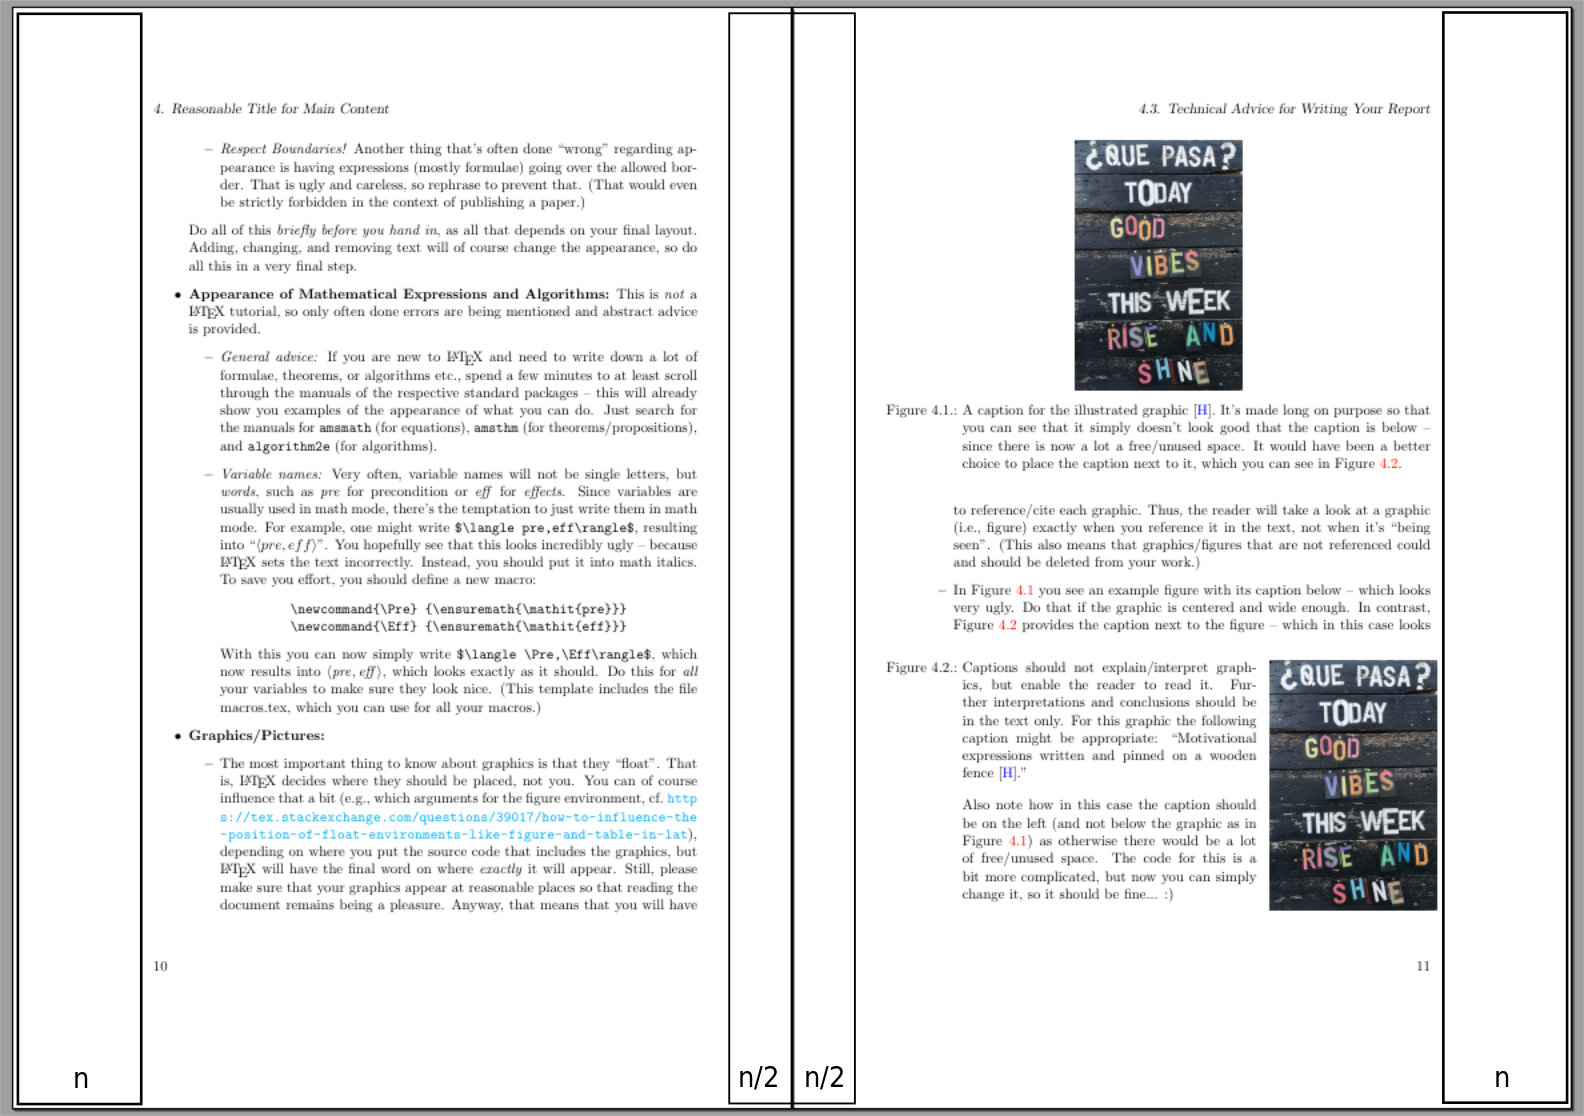
\includegraphics[width=.55\textwidth]{figures/borders--annotated}
  \caption{Illustration showing why page borders flip.\label{fig:pageBorders}}
\end{figure}%

                    % appendix 2


% literature
\bibliographystyle{anuthesis} % or plainnat or whatever
\cleardoublepage\phantomsection
% see https://tex.stackexchange.com/questions/60556/link-to-bibliography-in-the-toc-fails
\bibliography{bib}
\end{document}
